


\begin{figure}[t]
     \centering
     \begin{subfigure}[b]{0.3\textwidth}
         \centering
         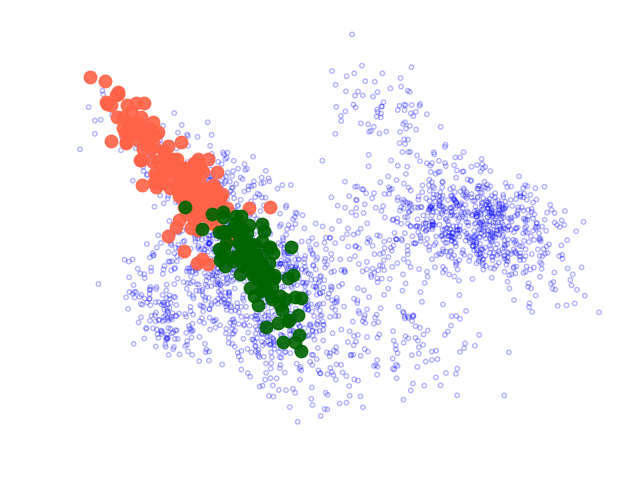
\includegraphics[width=\textwidth]{PaperB/figures_and_tables/latent_space_visualizations/apples_new/pca_latent_apples_vcca_xi_seed2.png}
         \caption{VCCA$_{x i}$}
         \label{fig:pca_vcca_xi_apples}
     \end{subfigure} 
     \begin{subfigure}[b]{0.3\textwidth}
         \centering
         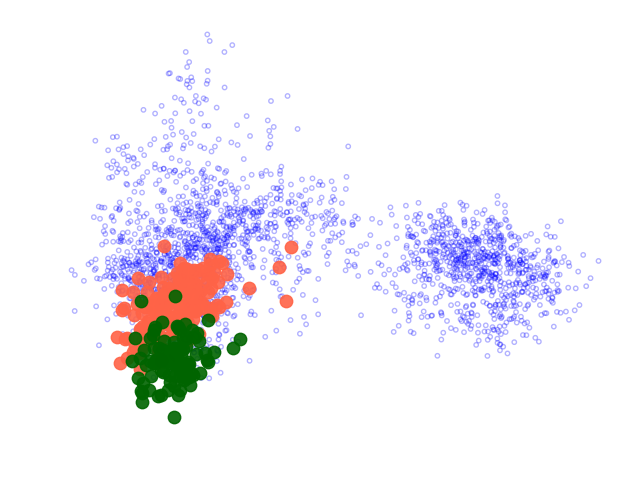
\includegraphics[width=\textwidth]{PaperB/figures_and_tables/latent_space_visualizations/apples_new/pca_latent_apples_vcca_xw_seed2.png}
         \caption{VCCA$_{x w}$}
         \label{fig:pca_vcca_xw_apples}
     \end{subfigure} 
     \begin{subfigure}[b]{0.3\textwidth}
         \centering
         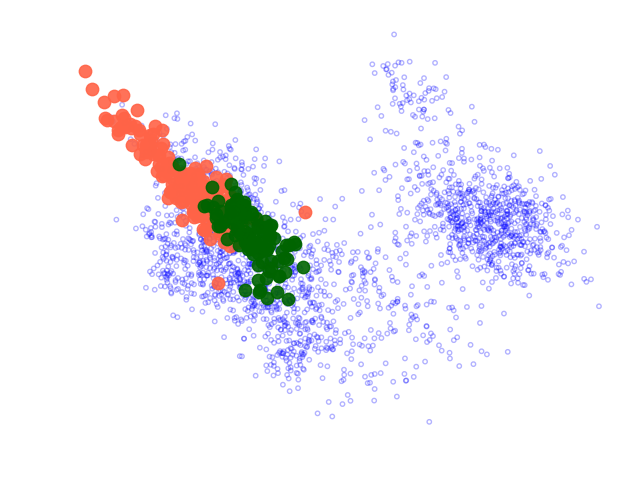
\includegraphics[width=\textwidth]{PaperB/figures_and_tables/latent_space_visualizations/apples_new/pca_latent_apples_vcca_xiw_seed2.png}
         \caption{VCCA$_{x i w}$}
         \label{fig:pca_vcca_xiw_apples}
     \end{subfigure} \\
     \begin{subfigure}[b]{0.3\textwidth}
         \centering
         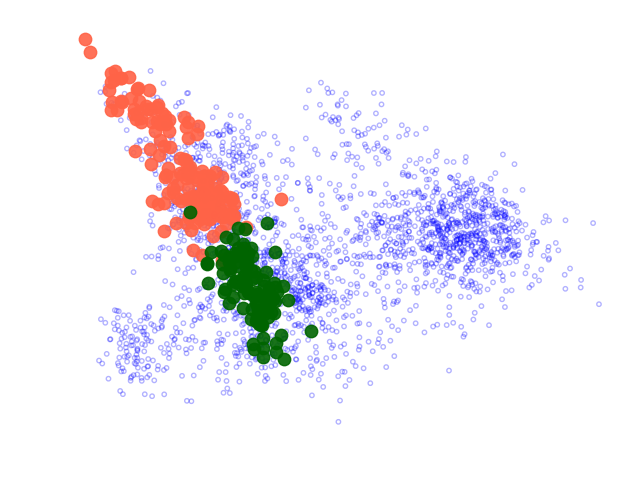
\includegraphics[width=\textwidth]{PaperB/figures_and_tables/latent_space_visualizations/apples_new/pca_latent_apples_vcca_xiy_seed2.png}
         \caption{VCCA$_{x i y}$}
         \label{fig:pca_vcca_xiy_apples}
     \end{subfigure} 
     \begin{subfigure}[b]{0.3\textwidth}
         \centering
         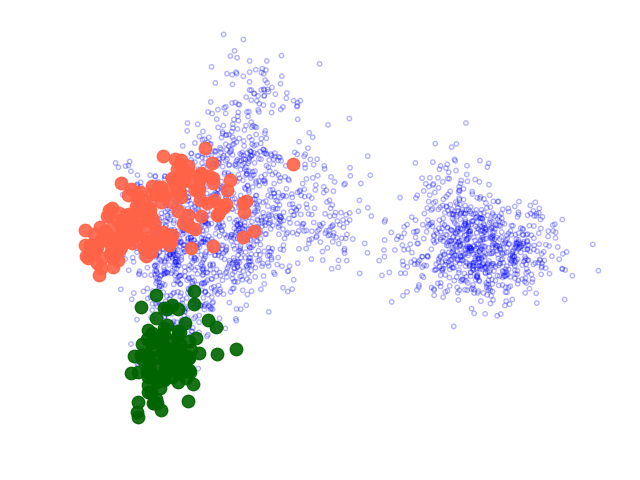
\includegraphics[width=\textwidth]{PaperB/figures_and_tables/latent_space_visualizations/apples_new/pca_latent_apples_vcca_xwy_seed2.png}
         \caption{VCCA$_{x w y}$}
         \label{fig:pca_vcca_xwy_apples}
     \end{subfigure} 
     \begin{subfigure}[b]{0.3\textwidth}
         \centering
         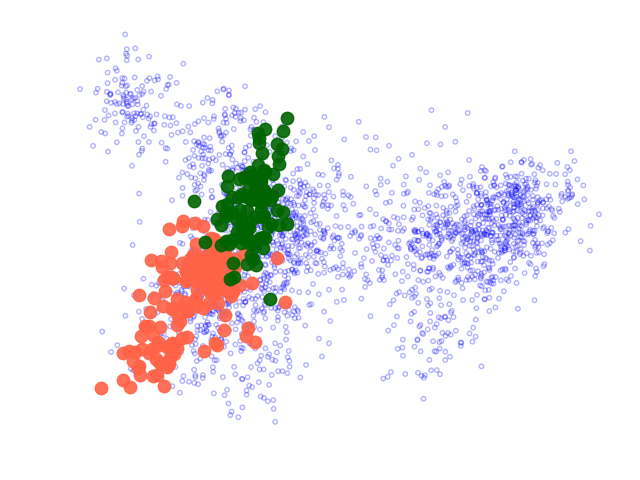
\includegraphics[width=\textwidth]{PaperB/figures_and_tables/latent_space_visualizations/apples_new/pca_latent_apples_vcca_xiwy_seed2.png}
         \caption{VCCA$_{x i w y}$}
         \label{fig:pca_vcca_xiwy_apples}
     \end{subfigure} 
    \caption{Visualizations of the latent representations $\mu_{z}$ of the red and green apples in the Grocery Store dataset. The red points correspond to the red apple classes, while the green points correspond to the green apple. The blue points correspond to the other grocery items. 
    %Abbreviations: VCCA, Variational Canonical Correlation Analysis.
    }
    \label{fig:2d_visualizations_pca_apples}
\end{figure}
